% !TEX ROOT = ersti.tex
\setboolean{druckversion}{true}
%\usepackage[x-1a]{pdfx/pdfx}
%\newcommand{\altstadtkarte}{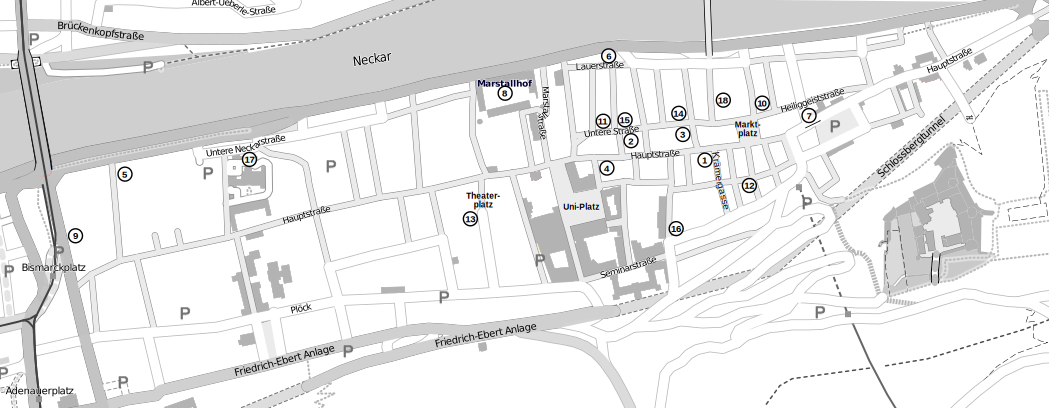
\includegraphics[width=120mm, clip, trim=1mm 0mm 15mm 0mm]{bilder/altstadt.pdf}} % Raster
%\newcommand{\altstadtkarte}{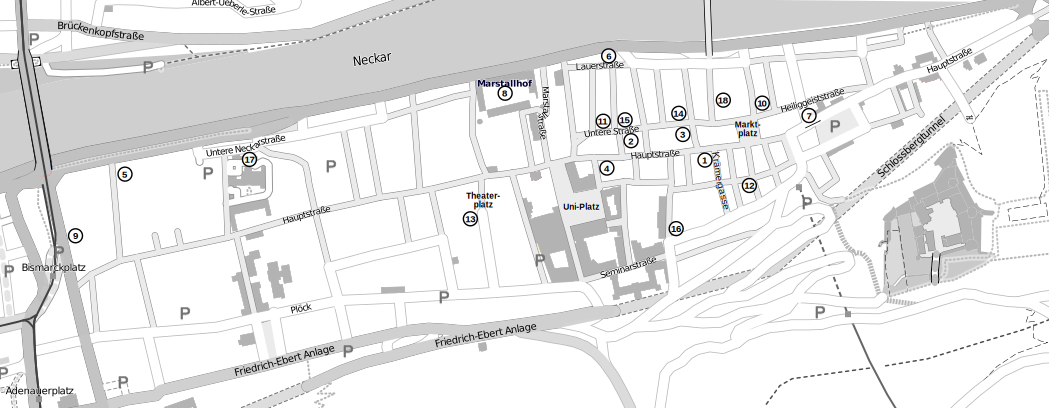
\includegraphics[width=120mm, trim=6mm 0mm 100mm 0mm, clip]{bilder/altstadt.pdf}} % Vektor
\newcommand{\altstadtkarte}{\includegraphics[width=\textwidth, trim=10mm 0mm 80mm 0mm, clip]{bilder/altstadt_cmyk.pdf}} % Vektor
\newcommand{\coverimage}{cover/ErstiInfo_Cover_2016_5mm_Bleed_CMYK.pdf}
%\newcommand{\coverimage}{cover/ErstiInfo_Cover_2016_no_Bleed.pdf}
\newcommand{\festimage}{cover/muphirho_druck.pdf}
\newcommand{\nhfkarte}{cover/nhf_cmyk.pdf}
\newcommand{\philwegkarte}{cover/philweg_cmyk.pdf}
\usepackage[draft]{hyperref}

% Sonderdruckfarben!
\iftrue
\usepackage[hks,pantone]{spotcolor}
\SetPageColorSpace{PANTONE}
\definecolor{sectiontextfarbe}  {spotcolor}{PANTONE363PC,1.0}
\definecolor{kapitelhintergrund}{spotcolor}{PANTONE363PC,1.0}
\else
\definecolor{kapitelhintergrund}{RGB}{207,207,207}
\definecolor{sectiontextfarbe}{RGB}{100,100,100}
\fi

% Erzeuge durch vier teilbare Seitenanzahl für den Druck.
\input{durch4teilbar}

% Trim options
%\setstocksize{307mm}{215mm}
%\settrimmedsize{297mm}{210mm}{*}
%\settrims{5mm}{0mm}
%\checkandfixthelayout
\showtrimsoff
\trimLmarks
%\trimFrame
%\quarkmarks
